\vspace*{2em}
Let's define what an \textit{articulation point} is. We say that a vertex $V$ in a graph $G$ with $C$
connected components is an \textit{articulation point} if its removal increases the number of connected components of $G$.
In other words, let $C'$ be the number of connected components after removing vertex $V$, if $C' > C$ then $V$ is an \textit{articulation point}.

\begin{figure}[H]
  \centering
  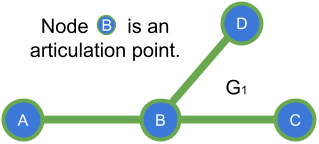
\includegraphics[width=0.3\textwidth]{"Images/Graph Theory/Articulation Points And Bridges/1.png"}
\end{figure}

\subsubsection*{How to find articulation points?}
\bullet Naive approach $O(V * (V + E))$

\begin{minted}{ruby}
for every vertex V in the graph G do
    Remove V from G
    if the number of connected components increases then V is an articulation point
    Add V back to G
\end{minted}